% \documentclass{book}

\documentclass[12pt]{article}
\usepackage[pdfborder={0 0 0.5 [3 2]}]{hyperref}%
\usepackage[left=1in,right=1in,top=1in,bottom=1in]{geometry}%
\usepackage[shortalphabetic]{amsrefs}%
\usepackage{amsmath}
\usepackage{enumerate}
\usepackage{enumitem}
\usepackage{amssymb}                
\usepackage{amsmath}                
\usepackage{amsfonts}
\usepackage{amsthm}
\usepackage{bbm}
\usepackage[table,xcdraw]{xcolor}
\usepackage{tikz}
\usepackage{float}
\usepackage{svg}
\usepackage{mathtools}
\usepackage{cool}
\usepackage{url}
\usepackage{graphicx,epsfig}
\usepackage{makecell}
\usepackage{array}

\graphicspath{ {images/} }
\renewcommand{\arraystretch}{3}

\begin{document}

\title{}
\author{\vspace{-10ex} }

\begin{center}
{\LARGE APMA 1650 -- Midterm 1}\\
\vspace{5mm}
{\large Wednesday, July 13, 2016 }\\
\vspace{10mm}
{\large Name: }
\vspace{3cm}

\begin{figure}[H]
\centering
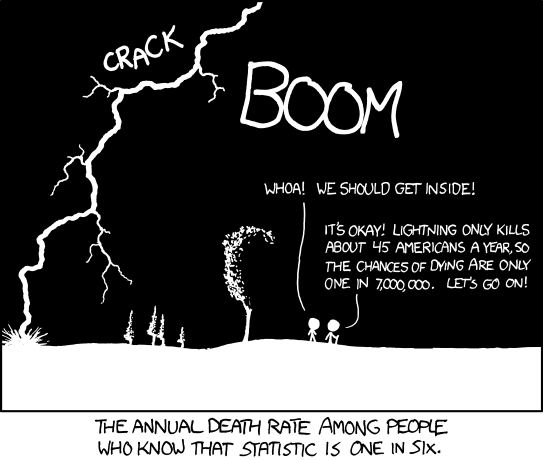
\includegraphics[width=15cm]{xkcd1}
\end{figure}
% {\large Due Tuesday, July 5, 2016}\\
% \vspace{5mm}
\end{center}
\pagebreak

\begin{center}
{\LARGE Instructions}\\
\vspace{5mm}
\end{center}

\begin{itemize}
\item The exams begins at 1:00 pm and ends at 3:00 pm. You have 2 hours to complete the exam.
\item You may use a calculator if you wish (although the exam is designed to be done without one, so I am not sure how helpful one will be). Other electronic devices may not be used and must be stowed beneath the seat in front of you or in the overhead compartment for the duration of the exam. You may not use any books or notes. 
\item Write all answers in the space below the question. If you need more space, feel free to use the back of the page.
\item Correct expressions are sufficient. You do not need to simplify your answers. You can leave answers in terms of binomial coefficients such as $\binom{64}{5}$, exponents such as $(1/2)^{10}$ or $2^{16}$, and factorials such as $12!$.
\item There are 5 questions. Each question is worth 10 points. Partial credit will be given for partially correct answers.
\item Unless you have found an error on the exam, in the interest of fairness, the exam proctor will likely not answer any questions you have about the test.
\item All answers must be fully justified. Show all of your work. Points will be deducted for unjustified answers.
\item I recommend you look through the entire exam first before answering any questions. That way you can start with the questions you find to be easiest.
\item The list of the common probability distributions, together with their pmfs/densities, expected values, and variances, is attached to the back of the exam.
\end{itemize}

\begin{figure}[H]
\centering
\label{my-label}
\begin{tabular}{|l|l|l|l|l|l|l|}
\hline
Problem & $\:\:1\:\:$ & $\:\:2\:\:$ & $\:\:3\:\:$ & $\:\:4\:\:$ & $\:\:5\:\:$ & Total \\ \hline
Points  &   &   &   &   &   &       \\ \hline
\end{tabular}
\end{figure}

\pagebreak

\begin{enumerate}
\item (10 points) 12 Brown undergraduate students -- 6 sophomores and 6 juniors -- enter the housing lottery. Suppose the students will live together in triples (groups of three) and are grouped into these triples uniformly at random.
\begin{enumerate}
\item How many possible arrangements are there of the 12 students into these triples?
\item What is the probability that no triple contains both sophomores and juniors? 
\end{enumerate}

\pagebreak

\item (10 points) Your friend has a bag of 3 six-sided dice. One of the dice is loaded so that the probability that it rolls a 6 is 1/2 (the rest of the numbers are rolled uniformly at random). The remaining two dice are standard, fair dice. You draw one of the dice from the bag uniformly at random and roll it.
\begin{enumerate}
\item If your roll is a 6, what is the probability that you rolled the unfair die?
\item If you then roll the same die again, what is the probability that it will roll a 6?
\end{enumerate} 

\pagebreak

\item (10 points) The ICERM building downtown has 11 floors (numbered 1 - 11). Suppose $m$ people enter the elevator on floor 1 and each one independently and uniformly at random chooses a floor between 2 and 11 (inclusive). What is the expected number of stops of the elevator?

\pagebreak

\item (10 points) You have two bags of marbles. Bag 1 contains 1 white marble and 5 red marbles. Bag 2 contains 5 white marbles and 1 red marble. You remove a marble uniformly at random from bag 1 and put it into bag 2. Then you remove a marble uniformly at random from bag 2 and put it back into bag 1. You do not look at the marble either time. At the end of this, what is the probability that the two bags have their original configurations (i.e. Bag 1 contains 1 white and 5 red marbles, Bag 2 contains 5 white and 1 red marbles)?

\pagebreak

\item (10 points) The Red Rose Tea company sells boxes of tea. Each box comes with a collectible figurine! There are $n$ total figurines, which are distributed uniformly at random in the boxes. You have already collected $m$ of them.
\begin{enumerate}
\item Suppose you buy $b$ boxes of tea. What is the probability that at least one of them contains a new figurine?
\item What is the expected number of boxes you need to buy until you get a new figurine?
\item What is the expected number of boxes you need to buy until you have collected all the figurines? 
\end{enumerate}

\end{enumerate}

\pagebreak


\begin{figure}[H]
\caption{Discrete Distributions}
\begin{tabular}{l c c c c}
\hline
Distribution & Parameters & Probability Mass Function (pmf) & Mean & Variance \\
\hline
Binomial & $n, p$ & \makecell{ $\displaystyle p(y) = \binom{n}{y}p^y(1-p)^{n-y}$\\$ \displaystyle y = 0, 1, \dots, n$} & $np$ & $np(1-p)$ \\
Geometric & $p$ & \makecell{ $\displaystyle p(y) = (1-p)^{y-1}p$ \\ $y = 1, 2, \dots$} & $ \displaystyle \frac{1}{p}$ & $\displaystyle \frac{1 - p}{p^2}$ \\
Poisson & $\lambda$ & \makecell{ $\displaystyle p(y) = \frac{e^{-\lambda} \lambda^y }{y!}$ \\ $y = 0, 1, 2, \dots$ } & $\lambda$ & $\lambda$ \\
\end{tabular}
\end{figure}

\vspace{2cm}

\begin{figure}[H]
\caption{Continuous Distributions}
\begin{tabular}{l c c c c}
\hline
Distribution & Parameters & Probability Density Function (pdf) & Mean & Variance \\
\hline
Uniform & $a, b$ & \makecell{ $\displaystyle f(y) = \frac{1}{b-a}$ \\ $a \leq y \leq b$ }& $\displaystyle \frac{a + b}{2}$ & $\displaystyle \frac{(b - a)^2}{12}$ \\
Exponential & $\lambda$ & \makecell{ $\displaystyle f(y) = \lambda e^{-\lambda y}$ \\ $0 \leq y < \infty$} & $\displaystyle \frac{1}{\lambda}$ & $\displaystyle \frac{1}{\lambda^2}$ \\
Normal & $\mu, \sigma$ & $\displaystyle f(y) = \frac{1}{\sqrt{2 \pi}\sigma}e^{- \frac{(y - \mu)^2}{2 \sigma^2}}$ & $\mu$ & $\sigma^2$ \\
Standard Normal & none & $\displaystyle f(y) = \frac{1}{\sqrt{2 \pi}}e^{- \frac{y^2}{2}}$ & $0$ & $1$ \\
\end{tabular}
\end{figure}

\end{document}

